\section{Determine the strength of a poker hand}

\subsection{Introduction}
There are different ways of evaluating the strength of a poker hand. One way is to create a formula (e.g. chen formula), another way could be to estimate the  probability of the hand ending up being the winning hand. We chose to use probability since other major poker sites uses probability to determine the strength of a poker hand. To estimate the probability we use the Monte Carlo method as it is the most widely used method for calculating poker statistics. 

\subsection{Monte Carlo method}
The Monte Carlo method can be used to calculate a probability distribution for domain. This is done by creating a large amount of simulations with random inputs within a range of allowed inputs. These simulations are also called Monte Carlo simulations. The more simulations that are performed the more accurate will the result be due to the large numbers law. 

When designing our Monte Carlo method we had the following requirements:
\begin{enumerate}
\item It should be able to return the probability for any poker state with up to ten players.
\item It should have an error of one percent at max.
\item It should calculate the probability in less than five seconds.
\end{enumerate}

To find out if the result is correct we compared our result to the results of other sources.

\subsection{Determine the number of simulations}
The only challenge we had when implementing the Monte Carlo method was to determine the number simulations. The number of simulations had a trade-off. The more simulations the calculations and time was needed but at the same time the more precise the result would get. 

To find right amount of simulations we created a test where we changed the number of simulations to see how it would affect the time and probability.

It calculates the probability of winning with a pair of jacks against a single opponent. Other sources estimated the probability to 0,771.
We plotted the results of running 50 test with 1000, 10.000 and 50.000 simulations. 

\begin{figure}[h!]
  \center
    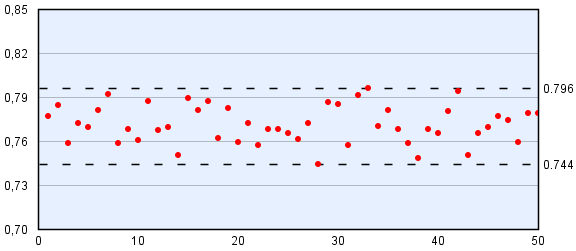
\includegraphics[scale=0.775]{images/MonteCarlo/1k.png}
  \caption{Result of Monte Carlo methods with 1000 simulations}
\end{figure}

\begin{figure}[h!]
  \center
    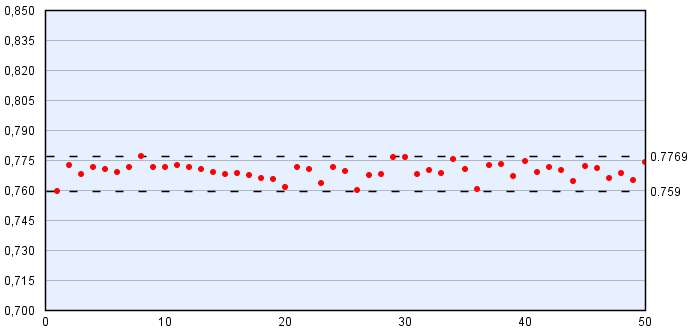
\includegraphics[scale=0.775]{images/MonteCarlo/10k.png}
  \caption{Result of Monte Carlo methods with 10.000 simulations}
\end{figure}

\begin{figure}[h!]
  \center
    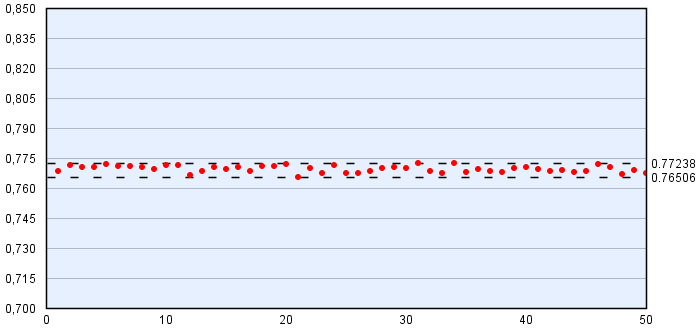
\includegraphics[scale=0.775]{images/MonteCarlo/50k.png}
  \caption{Result of Monte Carlo methods with 50.000 simulations}
\end{figure}

From the tests we found the maximum difference between the 50 results and the maximum difference from the expected result.

\vspace{4mm}
\begin{tabular}{ | l | l | l | l | }
  \hline
  simulations & max difference (\%) & max error (\%) & time (seconds) \\
  \hline                       
  1000 & 5,2 & 2,7 & 0,03 \\
  10.000 & 2,2 & 1,5 &  0,22\\
  50.000 & 0,9 & 0,7 & 0,82\\
  \hline  
\end{tabular}
\vspace{4mm}

We settled for 50.000 as the number of simulations for our Monte Carlo method. This satisfied our requirements.

\subsection{Test}


\subsection{Discussion}

\subsection{Conclusion}